\begin{frame}{Null-text Inversion: Example}
    \begin{figure}[t]
        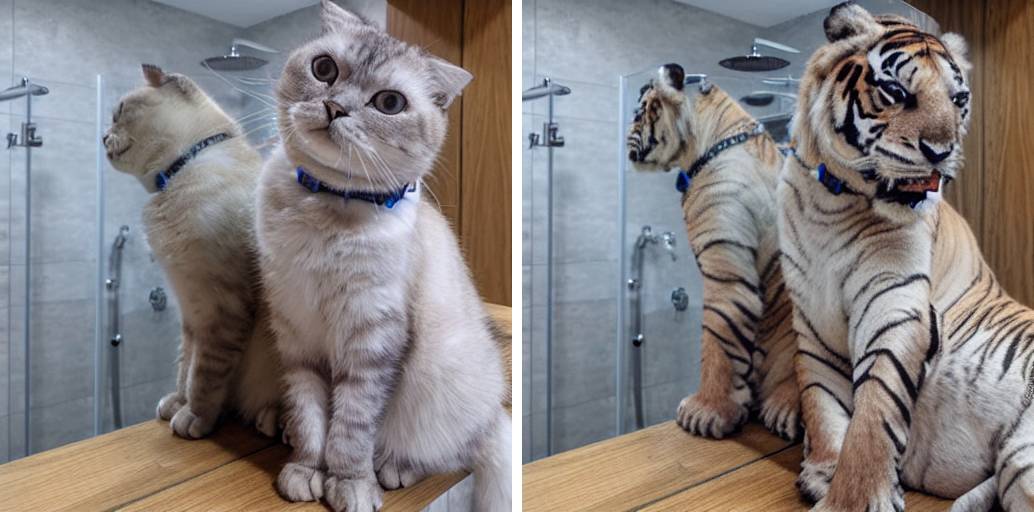
\includegraphics[width=.5\textwidth]{../../../resources/stereodiffusion/conditioning/left/TRAIN-TEST_cat_images_inference.png}
        \caption{Example of image editing using Null-text Inversion \cite{mokady2023null}}
    \end{figure}
    \begin{center}
        "a cat sitting next to a mirror" $\rightarrow$ "a tiger sitting next to a mirror"
    \end{center}
\end{frame}

\begin{frame}{Generated Image Pair: Without vs With Guidance Prompt}
    \begin{columns}
        \begin{column}{0.5\textwidth}
            \begin{figure}[t]
                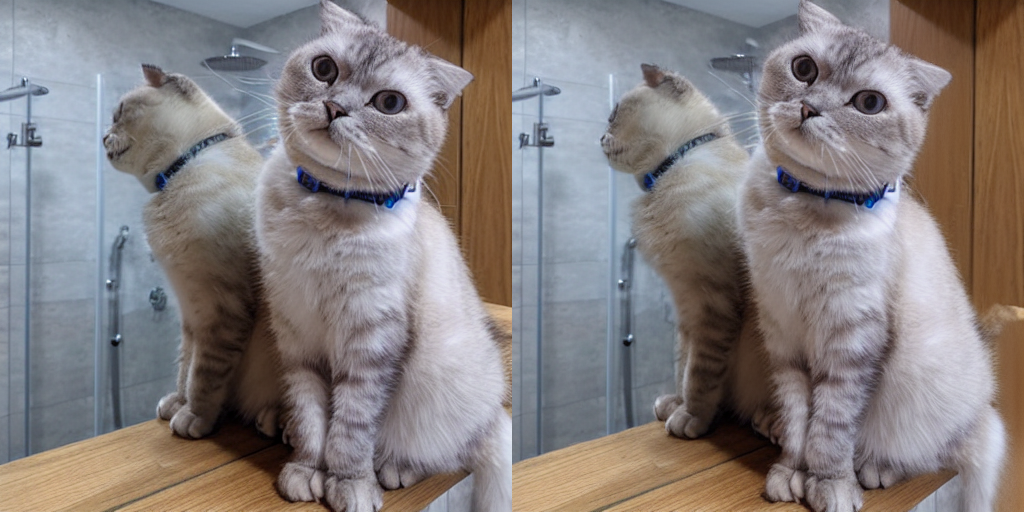
\includegraphics[width=\textwidth]{../../../resources/stereodiffusion/TRAIN-TEST_cat_DPT-disparity_image_pair.png}
                \caption{Without prompt}
            \end{figure}
        \end{column}
        \begin{column}{0.5\textwidth}
            \begin{figure}[t]
                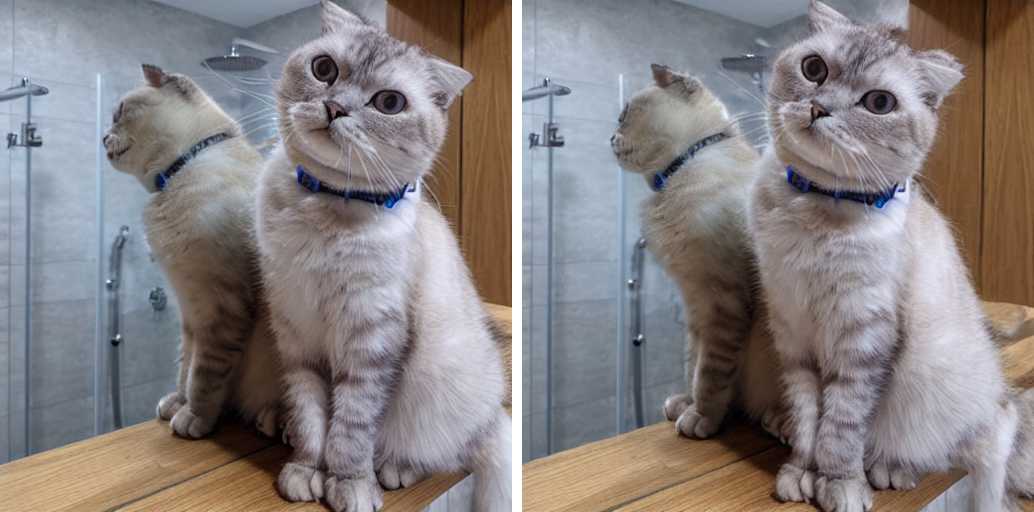
\includegraphics[width=\textwidth]{../../../resources/stereodiffusion/conditioning/stereo-bnattention/deblurred/TRAIN-TEST_cat_images_inference.png}
                \caption{With prompt}
            \end{figure}
        \end{column}
    \end{columns}
    \begin{center}
        Prompt:\\
        "a cat sitting next to a mirror, captured by a stereo camera with baseline distance \mono{baseline} and focal length \mono{focal\_length}"
    \end{center}
\end{frame}

\begin{frame}{Attention scores for the guidance prompt}
    \begin{figure}[t]
        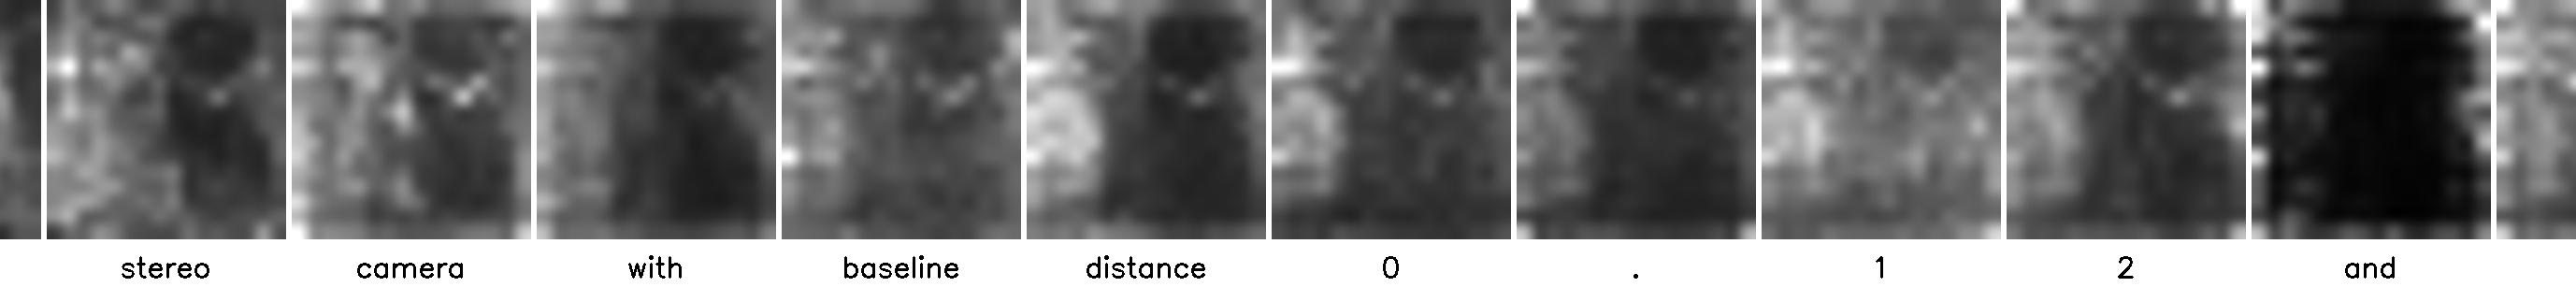
\includegraphics[width=\textwidth]{images/attention_scores_cut.png}
        \caption{Attention scores for the tokens corresponding to the baseline distance...}
    \end{figure}
\end{frame}

\begin{frame}{Cross- vs Uni/Bi-directional Attention: Generated Image Pair}
    \begin{columns}
        \begin{column}{0.5\textwidth}
            \begin{figure}[t]
                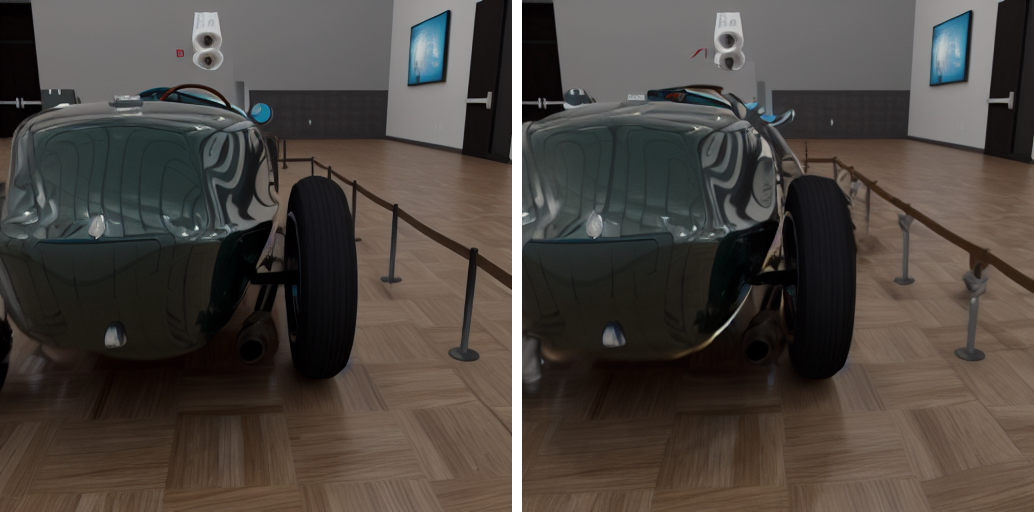
\includegraphics[width=\textwidth]{../../../resources/stereodiffusion/conditioning/stereo-attention/deblurred/TRAIN-TEST_car_images_inference.png}
                \caption{StereoDiffusion with Cross-Attention}
            \end{figure}
        \end{column}
        \begin{column}{0.5\textwidth}
            \begin{figure}[t]
                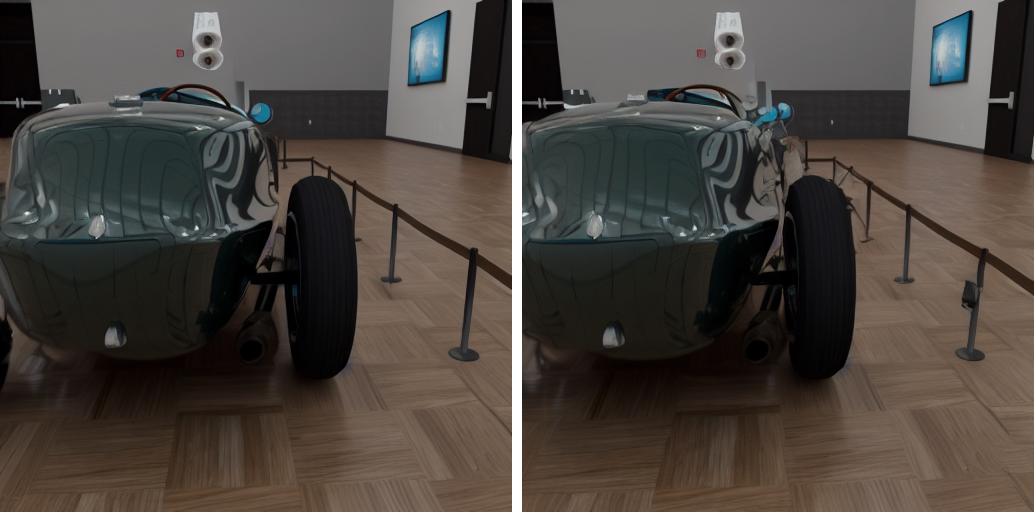
\includegraphics[width=\textwidth]{../../../resources/stereodiffusion/conditioning/stereo-bnattention/deblurred/TRAIN-TEST_car_images_inference.png}
                \caption{StereoDiffusion with Uni-directional Attention}
            \end{figure}
        \end{column}
    \end{columns}
\end{frame}

\begin{frame}{Cross- vs Uni/Bi-directional Attention: Attention Scores}
    \begin{figure}[t]
        
\includegraphics[width=3.8\textwidth]{../../../resources/stereodiffusion/conditioning/stereo-attention/deblurred/TRAIN-TEST_car_images_cond_cross-attention.png}
        \caption{Aggregated Cross-Attention scores}
    \end{figure}
    \begin{figure}[t]
        
\includegraphics[width=3.8\textwidth]{../../../resources/stereodiffusion/conditioning/stereo-bnattention/deblurred/TRAIN-TEST_car_images_cond_cross-attention.png}
        \caption{Aggregated Uni-directional Attention scores}
    \end{figure}
\end{frame}

\begin{frame}{Deblurring: Generated Image Pair}
    \begin{columns}
        \begin{column}{0.5\textwidth}
            \begin{figure}[t]
                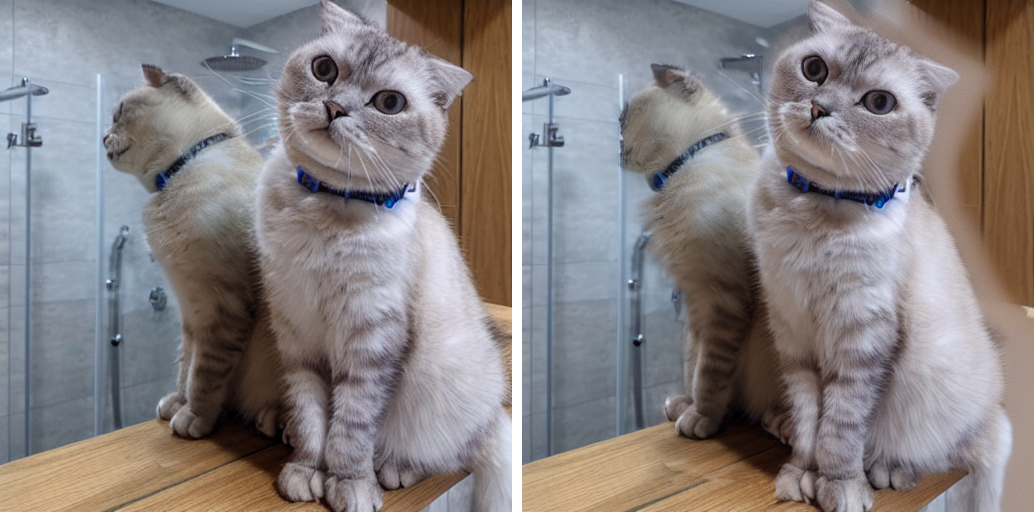
\includegraphics[width=\textwidth]{../../../resources/stereodiffusion/conditioning/stereo-attention/TRAIN-TEST_cat_images_inference.png}
                \caption{StereoDiffusion without deblurring}
            \end{figure}
        \end{column}
        \begin{column}{0.5\textwidth}
            \begin{figure}[t]
                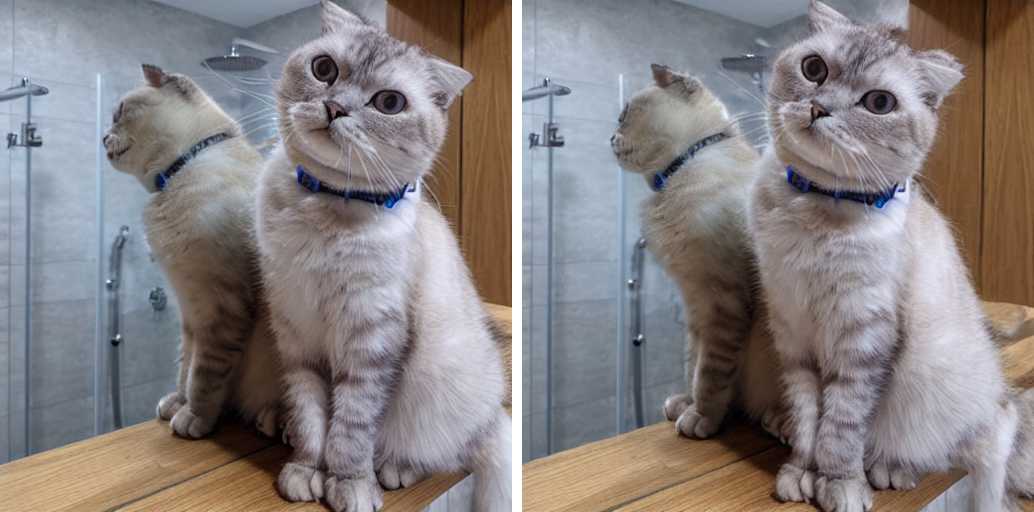
\includegraphics[width=\textwidth]{../../../resources/stereodiffusion/conditioning/stereo-bnattention/deblurred/TRAIN-TEST_cat_images_inference.png}
                \caption{StereoDiffusion with deblurring}
            \end{figure}
        \end{column}
    \end{columns}
\end{frame}

\begin{frame}{Deblurring in Latent Space}
    \begin{columns}
        \begin{column}{0.5\textwidth}
            \begin{figure}[t]
                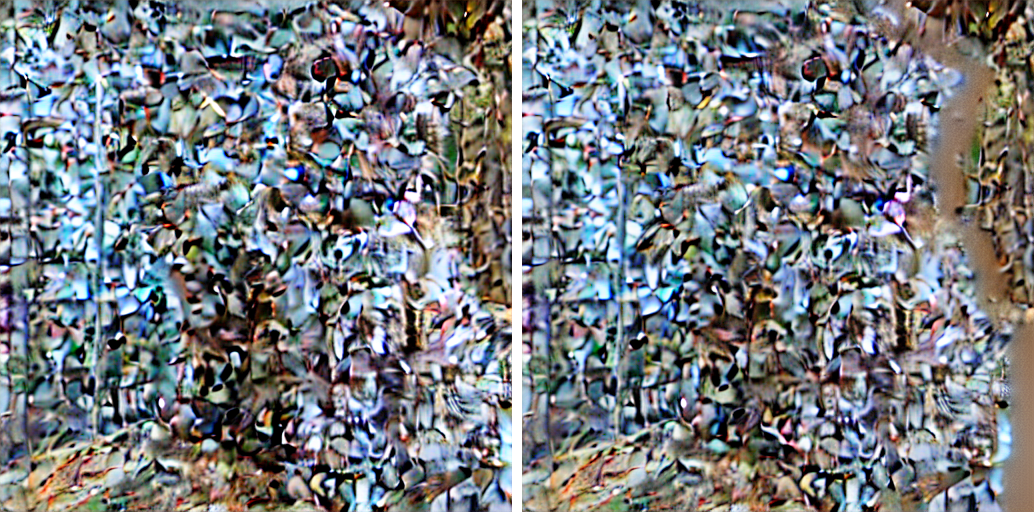
\includegraphics[width=\textwidth]{../../../resources/stereodiffusion/conditioning/stereo-attention/TRAIN-TEST_cat_latents_at_t=581.png}
                \caption{Latent state without deblurring}
            \end{figure}
        \end{column}
        \begin{column}{0.5\textwidth}
            \begin{figure}[t]
                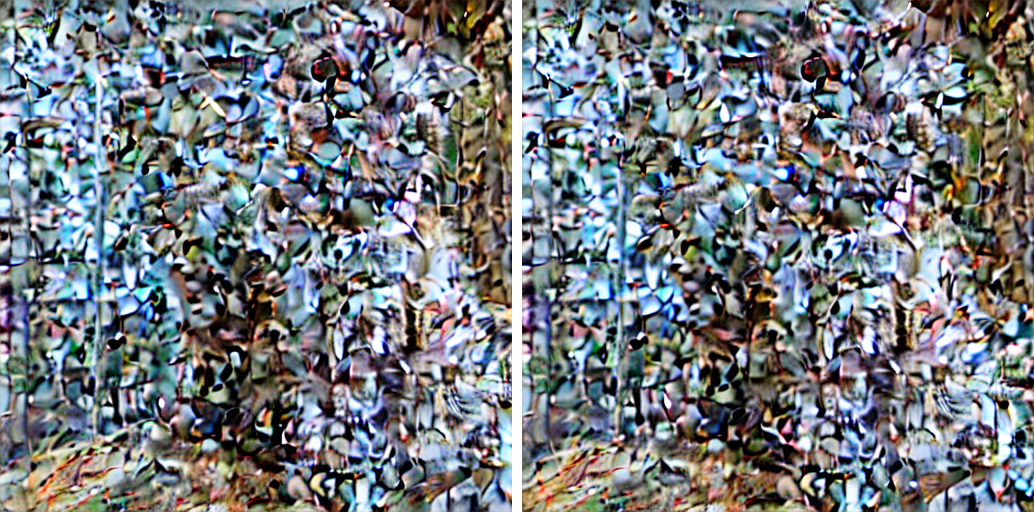
\includegraphics[width=\textwidth]{../../../resources/stereodiffusion/conditioning/stereo-bnattention/deblurred/TRAIN-TEST_cat_latents_at_t=581.png}
                \caption{Latent state with deblurring}
            \end{figure}
        \end{column}
    \end{columns}
\end{frame}

\begin{frame}{Disparity Map: DPT with estimated sensor data vs DPT}
    \begin{columns}
        \begin{column}{0.5\textwidth}
            \begin{figure}[t]
                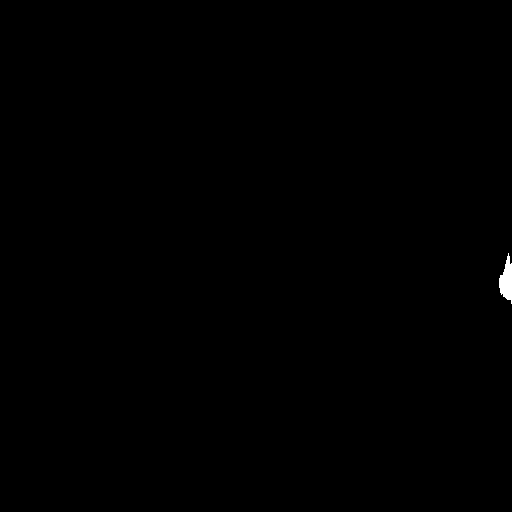
\includegraphics[width=.75\textwidth]{../../../resources/stereodiffusion/TRAIN-TEST_cat_DPT-depth-to-disparity_B0.12_f39.1.png}
                \caption{DPT depth with estimated sensor data}
            \end{figure}
        \end{column}
        \begin{column}{0.5\textwidth}
            \begin{figure}[t]
                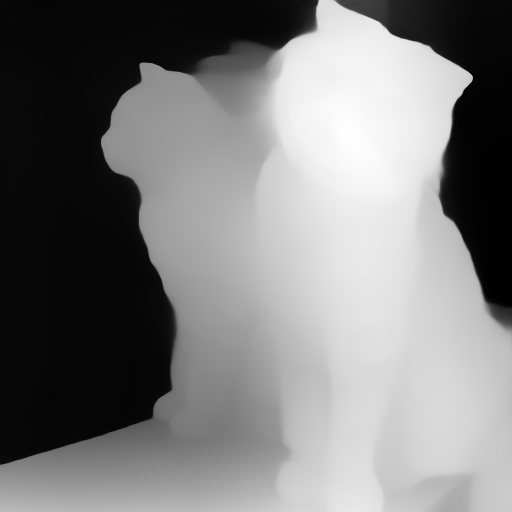
\includegraphics[width=.75\textwidth]{../../../resources/stereodiffusion/TRAIN-TEST_cat_DPT-disparity.png}
                \caption{DPT disparity}
            \end{figure}
        \end{column}
    \end{columns}
\end{frame}

\begin{frame}{Disparity Map: DPT with real sensor data vs DPT}
    \begin{columns}
        \begin{column}{0.5\textwidth}
            \begin{figure}[t]
                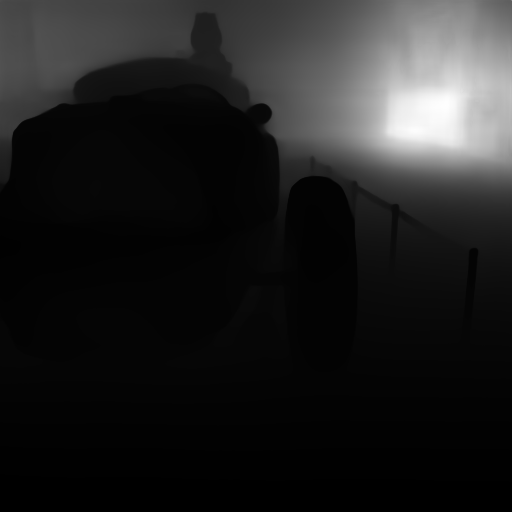
\includegraphics[width=.75\textwidth]{../../../resources/stereodiffusion/TRAIN-TEST_car_DPT-depth-to-disparity_B0.12_f39.111461135307415.png}
                \caption{DPT depth with real sensor data}
            \end{figure}
        \end{column}
        \begin{column}{0.5\textwidth}
            \begin{figure}[t]
                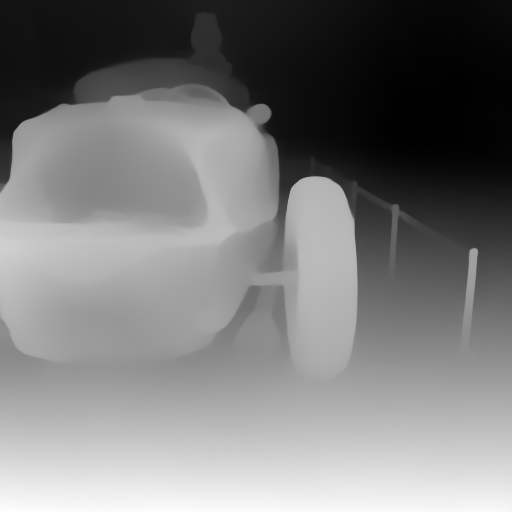
\includegraphics[width=.75\textwidth]{../../../resources/stereodiffusion/TRAIN-TEST_car_DPT-disparity.png}
                \caption{DPT disparity}
            \end{figure}
        \end{column}
    \end{columns}
\end{frame}

\begin{frame}{Disparity Map Histogram: DPT with real sensor data vs DPT}
    \begin{columns}
        \begin{column}{0.5\textwidth}
            \begin{figure}[t]
                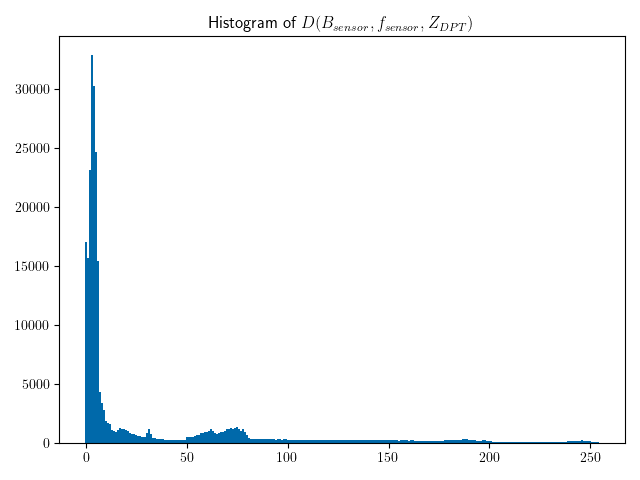
\includegraphics[width=.75\textwidth]{../../../resources/stereodiffusion/TRAIN-TEST_car_DPT-depth-to-disparity_hist_B0.12_f39.111461135307415.png}
                \caption{Histogram: DPT depth with real sensor data}
            \end{figure}
        \end{column}
        \begin{column}{0.5\textwidth}
            \begin{figure}[t]
                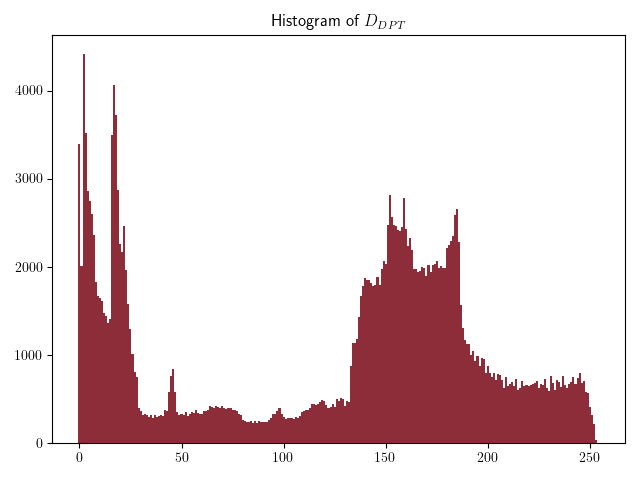
\includegraphics[width=.75\textwidth]{../../../resources/stereodiffusion/TRAIN-TEST_car_DPT-disparity_hist.png}
                \caption{Histogram: DPT disparity}
            \end{figure}
        \end{column}
    \end{columns}
\end{frame}

\begin{frame}{Preliminary Goals for the Evaluation}
    Evaluate StereoDiffusion with different alterations:
    \begin{itemize}
        \item (Fully vs. partly estimated disparity)
        \item Cross-Attention vs. *-directional Attention
        \item With vs. without prompt guidance
    \end{itemize}
    \bigskip
    Evaluation dataset:
    \begin{itemize}
        \item 1k samples, generated with Blender
        \item contains: stereo image pair, camera parameters, disparity map
    \end{itemize}
    \bigskip
    Nice-to-have:
    \begin{itemize}
        \item Which is better: fully vs. partly estimated disparity
    \end{itemize}
\end{frame}